\documentclass[../main-physics-workbook.tex]{subfiles}
\begin{document}

\setcounter{section}{7}
\subsection{Factors That Affect Projectile Trajectory}

\subsubsection{Trajectory, Hang Time, Max Height, and Range}

\fbox{\fbox{
\begin{minipage}{0.6\textwidth}
\textbf{Instructions}:
\vspace{-1ex}
\begin{center}
\begin{itemize}[itemsep=0pt]
    \item Go to \href{https://phet.colorado.edu/en/simulations/projectile-motion}{phet.colorado.edu/en/simulations/projectile-motion}
    \item Press play to enter the simulation.
    \item Click the fourth panel, called ``Lab''
    \smallskip
\end{itemize}
\end{center}
\end{minipage}%
\begin{minipage}{0.37\textwidth}
\centering
\includegraphics[height=2cm]{documents/figures/phet-projectile-play.png}
\hspace{2pt}
\includegraphics[height=2cm]{documents/figures/phet-projectile-lab.png}
\end{minipage}
}}


\begin{questions}
\question 
When you first open the Lab page, don't press anything on the screen. Now press the red fire button to launch a cannon ball. Read the values on the screen, or use the measuring tool to record these quantities:

\begin{parts}
\part What is the initial speed? \fillin[\SI{18}{m/s}][2cm]
\part What is the launch angle? \fillin[\ang{80}][2cm]
\part Measure the height at the apex. \fillin[\SI{16.02}{m}][2cm]
\part What is the hang time? \fillin[\SI{3.61}{s}][2cm]
\part What is the horizontal displacement of the projectile when it strikes ground? \fillin[\SI{11.3}{m}][2cm]
\end{parts}


\question \label{Q1}
Using the same initial speed of \SI{18}{m/s} and launch angle of \ang{80} above the horizontal, measure the range and height throughout the trajectory, at 0.4-second time intervals, and record your data in the table below.

\begin{center}
% \bgroup
% \def\arraystetch{3}
\begin{tabu}{|c|c|c|c|c|c|c|c|c|c|c|}
    \hline
    \textbf{time} (s) & 0.0 & 0.4 & 0.8 & 1.2 & 1.6 & 2.0 & 2.4 & 2.8 & 3.2 & 3.6 \\ \hline
    \ifprintanswers
        \rowfont{\color{red}}
    \else
        \rowfont{\color{white}}
    \fi
    \textcolor{black}{\textbf{range} (m)} & 0.00 & 1.25 & 2.5 & 3.75 & 5.0 & 6.25 & 7.5 & 8.75 & 10 & 11.25\\ \hline
    \ifprintanswers
        \rowfont{\color{red}}
    \else
        \rowfont{\color{white}}
    \fi
    \textcolor{black}{\textbf{height} (m)} & 0.00 & 6.31 & 11.04 & 14.21 & 15.81 & 15.83 & 14.29 & 11.18 & 6.5 & 0.25\\ \hline
\end{tabu}
% \egroup
\end{center}

\question \label{qdcpx}
The range is the horizontal position relative to the origin, and the height is the vertical position. 

\begin{parts}
\part Using your table from Question \ref{Q1}, make graphs of range vs. time and height vs. time. Note that both graphs are position vs. time graphs.

\begin{center}
\begin{tikzpicture}
    \begin{axis}[height=6cm,width=7cm,
        axis lines=left,
        ylabel={range (m)},
        xlabel={time (s)},
        ymin=0,ymax=12,
        xmin=0,xmax=4,
        ytick={0,2,...,12},
        xtick={0,1,...,4},
        minor x tick num=1,
        grid=both,
    ]
    \ifprintanswers
        \addplot[mark=*,red] coordinates {(0,0)(0.4,1.25)(0.8,2.5)(1.2,3.75)(1.6,5.0)(2.0,6.25)(2.4,7.5)(2.8,8.75)(3.2,10)(3.6,11.25)};
    \fi
    \end{axis}
\end{tikzpicture}
\hspace{5mm}
\begin{tikzpicture}
    \begin{axis}[height=6cm,width=7cm,
        axis lines=left,
        ylabel={height (m)},
        xlabel={time (s)},
        ymin=0,ymax=18,
        xmin=0,xmax=4,
        ytick={0,2,...,18},
        xtick={0,1,...,4},
        minor x tick num=1,
        grid=both,
    ]
    \ifprintanswers
        \addplot[mark=*,red] coordinates {(0,0)(0.4,6.31)(0.8,11.04)(1.2,14.21)(1.6,15.81)(2.0,15.83)(2.4,14.29)(2.8,11.18)(3.2,6.5)(3.6,0.25)};
    \fi
    \end{axis}
\end{tikzpicture}
\end{center}

\part What is the mathematical relationship between range and time in projectile motion?

\ifprintanswers
\else
\fillwithlines{1.5cm}
\fi

\begin{solution}
According to the graph, there is a linear relationship between range and time.
\end{solution}

\part What is the mathematical relationship between height and time in projectile motion?

\ifprintanswers
\else
\fillwithlines{1.5cm}
\fi

\begin{solution}
According to the graph, there is a quadratic (or parabolic) relationship between height and time.
\end{solution}

\end{parts}

\question \label{ZDSnl}
Using your table from Question \ref{Q1}, predict the time, range, and height for the projectile at three specific positions---the origin, the apex, and at maximum range. Then use the tool to measure the actual values.

\bigskip

\begin{minipage}{0.48\textwidth}
\centering

\textbf{My predictions}
\medskip

\begin{tabu}{|c|c|c|c|}
    \hline
    & origin & apex & max range \\ \hline
    \rowfont{\color{white}}
    \textcolor{black}{\textbf{time} (s)} & 0 & 1.81 & 3.61 \\ \hline
    \rowfont{\color{white}}
    \textcolor{black}{\textbf{range} (m)} & 0 & 5.65 & 11.3 \\ \hline
    \rowfont{\color{white}}
    \textcolor{black}{\textbf{height} (m)} & 0 & 16.02 & 0 \\ \hline
\end{tabu}
\end{minipage}%
\begin{minipage}{0.48\textwidth}
\centering

\textbf{Actual values}
\medskip

\begin{tabu}{|c|c|c|c|}
    \hline
    & origin & apex & max range \\ \hline
    \ifprintanswers
        \rowfont{\color{red}}
    \else
        \rowfont{\color{white}}
    \fi
    \textcolor{black}{\textbf{time} (s)} & 0 & 1.81 & 3.61 \\ \hline
    \ifprintanswers
        \rowfont{\color{red}}
    \else
        \rowfont{\color{white}}
    \fi
    \textcolor{black}{\textbf{range} (m)} & 0 & 5.65 & 11.3 \\ \hline
    \ifprintanswers
        \rowfont{\color{red}}
    \else
        \rowfont{\color{white}}
    \fi
    \textcolor{black}{\textbf{height} (m)} & 0 & 16.02 & 0 \\ \hline
\end{tabu}
\end{minipage}

\question
Give a real-world example of an object undergoing projectile motion. Then draw its trajectory and label the launch angle, apex, and maximum height.

\begin{solutionorbox}[5cm]
    Answers will vary.
\end{solutionorbox}

\question
What is projectile motion?
    
\begin{randomizechoices}
    \correctchoice The motion of an object projected into the air and moving under the influence of gravity.
    \choice The motion of an object projected into the air and moving independently of gravity.
    \choice The motion of an object projected only vertically upward into the air and moving under the influence of gravity.
    \choice The motion of an object projected only horizontally into the air and moving independently of gravity.
\end{randomizechoices}

\question
What is the shape of a trajectory?

\begin{randomizechoices}
    \correctchoice a parabola
    \choice an ellipse
    \choice a circle
    \choice a line
\end{randomizechoices}

\question
The point in a projectile's trajectory at which the object is at peak height is called

\begin{randomizechoices}
    \correctchoice the apex
    \choice the trajectory
    \choice the launch angle
    \choice the maximum range
\end{randomizechoices}

\question
What is the force experienced by a projectile after the initial force that launched it into the air?

\begin{randomizechoices}
    \choice The nuclear force
    \correctchoice The gravitational force
    \choice The electromagnetic force
    \choice The contact force
\end{randomizechoices}
\end{questions}


\subsubsection{How Initial Velocity, Launch Height, Launch Angle, and Mass Affect Motion}

\fbox{\fbox{
\begin{minipage}{0.6\textwidth}
\textbf{Instructions}:
\vspace{-1ex}
\begin{center}
\begin{itemize}[itemsep=0pt]
    \item Go to \href{https://phet.colorado.edu/en/simulations/projectile-motion}{phet.colorado.edu/en/simulations/projectile-motion}
    \item Press play to enter the simulation.
    \item Click the fourth panel, called ``Lab''
    \smallskip
\end{itemize}
\end{center}
\end{minipage}%
\begin{minipage}{0.37\textwidth}
\centering
\includegraphics[height=2cm]{documents/figures/phet-projectile-play.png}
\hspace{2pt}
\includegraphics[height=2cm]{documents/figures/phet-projectile-lab.png}
\end{minipage}
}}




\begin{questions}

\question
Let's explore how changing initial speed affects projectile trajectory. In the parts below, change \textit{only} the initial speed and leave all other parameters the same.

\begin{parts}
\part Fire the cannonball at the default values of \SI{18}{m/s} and \ang{80}. Then, fire a second cannonball at a lower speed of \SI{12}{m/s} and then a third at \SI{24}{m/s}. Sketch all three trajectories below.

\begin{center}
\begin{tikzpicture}
    \begin{axis}[height=7cm,width=8cm,
        axis lines=left,
        ylabel={$y$ (m)},
        y label style={rotate=-90},
        xlabel={$x$ (m)},
        ymin=0,ymax=30,
        xmin=0,xmax=22,
        ytick={0,3,...,30},
        xtick={0,2,...,22},
        minor x tick num=1,
        grid=both,
        %legend pos=outer north east,
    ]
    \ifprintanswers
        \addplot[domain=0:11.3,thick,red] {trajectoryequation(x,18,80)};
        \addlegendentry{$v_i = \SI{18}{m/s}$}
        \addplot[domain=0:5.02,thick,blue] {trajectoryequation(x,12,80)};
        \addlegendentry{$v_i = \SI{12}{m/s}$}
        \addplot[domain=0:20.08,thick,green!60!black] {trajectoryequation(x,24,80)};
        \addlegendentry{$v_i = \SI{24}{m/s}$}
    \fi
    \end{axis}
\end{tikzpicture}
\end{center}

\part How does changing the initial speed affect the trajectory, hang time, max height, and range of a projectile? Cite evidence from your graph and measurements from the simulation to support your answer.

\ifprintanswers
\else
\fillwithlines{4cm}
\fi

\begin{solution}
    The sketches in the previous part show that as the initial speed increases, the trajectory gets wider and taller, consistent with increasing range and apex height. The measuring tool records that hang time, max height, and range all increases as the initial speed increases.
\end{solution}
\end{parts}


\question
Locate the $\boldsymbol{+}$ symbol on the center of the cannon. Click-and-drag the $\boldsymbol{+}$ to change the cannon's launch height to 3 meters. Fire the projectile from this new height, with the same speed (\SI{18}{m/s}) and angle (\ang{80}) as before. 


\begin{parts}
\part Identify at least two differences in the trajectories of a projectile launched from a height of 3 meters and one launched from ground-level.

\ifprintanswers
\else
\fillwithlines{2cm}
\fi

\begin{solution}
The object has a greater hang time and higher apex when it is launched from 3 meters compared to ground level.
\end{solution}

\part Fire the cannon successively from launch heights of \SI{0}{m}, \SI{3}{m}, \SI{6}{m}, \SI{9}{m}, \SI{12}{m}, and \SI{15}{m}. Then sketch the six trajectories below. What similarities do you see? What differences?

\begin{center}
\begin{tikzpicture}
    \begin{axis}[height=7cm,width=7cm,
        axis lines=left,
        ylabel={$y$ (m)},
        y label style={rotate=-90},
        xlabel={$x$ (m)},
        ymin=0,ymax=33,
        xmin=0,xmax=14,
        ytick={0,3,...,33},
        xtick={0,2,...,14},
        minor x tick num=1,
        grid=both,
    ]
    \ifprintanswers
    \draw[dashed,gray,thick] (5.65,0) -- ++(0,33);
    \addplot[domain=0:11.3,thick,red] {trajectoryequation(x,18,80)};
    \addplot[domain=0:11.8,thick,red] {trajectoryequation(x,18,80) + 3};
    \addplot[domain=0:12.27,thick,red] {trajectoryequation(x,18,80) + 6};
    \addplot[domain=0:12.71,thick,red] {trajectoryequation(x,18,80) + 9};
    \addplot[domain=0:13.12,thick,red] {trajectoryequation(x,18,80) + 12};
    \addplot[domain=0:13.51,thick,red] {trajectoryequation(x,18,80) + 15};
    \fi
    \end{axis}
\end{tikzpicture}
\end{center}

\begin{solution}
All trajectories have the same general, parabolic shape. The apex of all trajectories occurs at the same horizontal position. However, the maximum range of the projectile increases as the initial launch height increases: a projectile can travel farther if it's launch height is increased. 
\end{solution}

\part How does changing the launch height affect the the trajectory, hang time, max height, and range of a projectile? Use evidence from previous parts to support your answer.

\ifprintanswers
\else
\fillwithlines{1.5cm}
\fi

\begin{solution}
    Increasing the launch height increases the height of the apex (though not its horizontal position), the hang time, and the maximum range. 
\end{solution}
\end{parts}


\question 
Click $\boldsymbol{\circlearrowleft}$ to reset default settings, and let's explore how changing the launch angle affects projectile motion.  In the parts below, change \textit{only} the launch angle and leave all other parameters the same.


\begin{parts}
\part With an initial speed at \SI{18}{m/s}, fire the projectile at the various angles shown below. Then record values for the hang time, the height of the apex, and the maximum range.

\begin{center}
\begin{tabu}{|c|c|c|c|c|c|c|c|c|c|}
    \hline
    \textbf{launch angle} & \ang{25} & \ang{30} & \ang{35} & \ang{40} & \ang{50} & \ang{60} & \ang{70} & \ang{80} & \ang{90} \\ \hline
    \ifprintanswers
        \rowfont{\color{red}}
    \else
        \rowfont{\color{white}}
    \fi
    \textcolor{black}{\textbf{hang time} (s)} & 1.55 & 1.83 & 2.10 & 2.36 & 2.81 & 3.18 & 3.45 & 3.61 & 3.67\\ \hline
    \ifprintanswers
        \rowfont{\color{red}}
    \else
        \rowfont{\color{white}}
    \fi
    \textcolor{black}{\textbf{apex height} (m)} & 2.95 & 4.13 & 5.43 & 6.82 & 9.69 & 12.38 & 14.58 & 16.02 & 16.51\\ \hline
    \ifprintanswers
        \rowfont{\color{red}}
    \else
        \rowfont{\color{white}}
    \fi
    \textcolor{black}{\textbf{maximum range} (m)} & 25.3 & 28.6 & 31.04 & 32.53 & 32.53 & 28.6 & 21.23 & 11.3 & 0.0 \\ \hline
\end{tabu}
\end{center}
\medskip

\part How does changing the launch angle affect the hang time and the apex height?

\ifprintanswers
\else
\fillwithlines{3cm}
\fi

\begin{solution}
    Increasing launch angle increases both the hang time and apex height.
\end{solution}


\part How does changing the launch angle affect the maximum range? (\textit{Caution}: Read the table carefully.)

\ifprintanswers
\else
\fillwithlines{3cm}
\fi


\begin{solution}
    Increasing launch angle from \ang{25} to \ang{40} degrees increases the maximum range, but increasing the angle from \ang{50} to \ang{90} decreases the maximum range. Therefore, the range first increases and then decreases as the launch angle increases.
\end{solution}


\part 
Of all angles available in the simulation, which angle yields the largest possible maximum range?
\fillin[\ang{45}][2cm]
\end{parts}

\question
You'll now explore how the mass of the projectile affects its trajectory. The mass of the projectile may be changed in the settings box in the upper right corner. 

\begin{parts}
\part Make a prediction for the following question. It's OK if your prediction turns out to be wrong.

\begin{center}
    \bfseries How does changing the projectile's mass affect its trajectory?
\end{center}

\textit{My prediction}:

\ifprintanswers
\else
\fillwithlines{3cm}
\fi

\begin{solution}
    Predictions will vary.
\end{solution}

\part Design and test an experiment in which \textit{only} the mass is varied and other parameters are left constant, so that you may test how mass affects the trajectory. Summarize your experiment and findings below.


\begin{solutionorbox}[10cm]
    Designs will vary.
\end{solutionorbox}


% \begin{solution}
%     The tables and graphs will be identical to the ones above.
% \end{solution}

\part How does changing mass affect the the trajectory, hang time, max height, and range of a projectile? Use evidence from your experiment to support your answer.

\ifprintanswers
\else
\fillwithlines{4cm}
\fi

\begin{solution}
    Mass does not affect a trajectory (assuming negligible air resistance).
\end{solution}
\end{parts}

\clearpage

\question
Decreasing the initial speed of a cannonball will cause the hang time to 

\begin{randomizechoices}
    \correctchoice decrease
    \choice increase
    \choice remain constant
    \choice become negative
\end{randomizechoices}

\question
Which of the following increases the apex height?

\begin{randomizechoices}
    \correctchoice increasing the initial speed
    \choice increasing the mass
    \choice decreasing the angle
    \choice decreasing the initial speed
\end{randomizechoices}

\question
The launch height affects all of the following EXCEPT

\begin{randomizechoices}
    \correctchoice the horizontal position of the apex
    \choice the vertical position of the apex
    \choice the hang time
    \choice the maximum range
\end{randomizechoices}

\question
How does increasing the launch angle affect the maximum range?

\begin{randomizechoices}[keeplast]
    \choice It increases the range.
    \choice It decreases the range.
    \choice It has no effect range.
    \correctchoice We can't know without knowing whether the angle is greater than or less than \ang{45}.
\end{randomizechoices}

\question
Increasing the mass will affect which of the following quantities?

\begin{randomizechoices}[keeplast]
    \choice hang time
    \choice maximum range
    \choice apex height
    \correctchoice none of the above
\end{randomizechoices}

\question
The maximum range of a projectile will increase if the launch angle changes from 

\begin{randomizechoices}
    \correctchoice \ang{25} to \ang{35}
    \choice \ang{40} to \ang{50}
    \choice \ang{60} to \ang{70}
    \choice \ang{75} to \ang{85}
\end{randomizechoices}

\question
To decrease the hang time, we can

\begin{randomizechoices}
    \correctchoice decrease the initial speed
    \choice increase the launch height
    \choice increase the launch angle from \ang{30} to \ang{60}
    \choice decrease the projectile mass
\end{randomizechoices}

\question
To maximize the range of a projectile, set the angle to 

\begin{randomizechoices}[keeplast,norandomize]
    \choice \ang{0}
    \correctchoice \ang{45}
    \choice \ang{90}
    \choice any angle
\end{randomizechoices}
\end{questions}

\clearpage

\subsection{Horizontally Launched Projectiles}

\subsubsection{Describing Vertical and Horizontal Motion Using Multiple Representations}

\clearpage
\subsubsection{Horizontal and Vertical Components with Vector Addition}

\fbox{\fbox{
\begin{minipage}{0.6\textwidth}
\textbf{Instructions}:
\vspace{-1ex}
\begin{center}
\begin{itemize}[itemsep=0pt]
    \item Go to \href{https://phet.colorado.edu/en/simulations/projectile-motion}{phet.colorado.edu/en/simulations/projectile-motion}
    \item Press play to enter the simulation.
    \item Click the second panel, called ``Vectors''
    \smallskip
\end{itemize}
\end{center}
\end{minipage}%
\begin{minipage}{0.37\textwidth}
\centering
\includegraphics[height=2cm]{documents/figures/phet-projectile-play.png}
\hspace{2pt}
\includegraphics[height=2cm]{documents/figures/phet-projectile-vectors.png}
\end{minipage}
}}

\begin{questions}
\question \label{KU3Mnf}
In this question we'll explore the horizontal and vertical components of the projectile's velocity.

\begin{parts}
\part Follow these steps:

\begin{itemize}
    \item Un-check the \texttt{Air Resistance} box. (Leave it blank.) Raise the cannon to a height of \SI{11}{m}.
    \item Set the launch angle to \ang{0} and the \texttt{Initial Speed} to \SI{10}{m/s}.
    \item Click the \texttt{Components} option, and check the \texttt{Velocity Vectors} box.
    \item Click the magnifying glass symbol to zoom out.
    \item Press \texttt{Pause} ({\small \faPause}).
    \item Press the \texttt{Fire} button.
    %The initial velocity, which is entirely horizontal is displayed. Notice that vertical velocity is not shown because it's zero.
    %\item Sketch the horizontal and vertical velocity vectors of this snapshot in a motion map. 
    \item To the right of the \texttt{Play} ({\small \faPlay}) button there is the \texttt{Step} button. Press the \texttt{Step} button several times to view the evolution of the horizontal and vertical velocity vectors across time.
    \item \label{LSagnx} Draw the the horizontal and vertical components of velocity in your motion map at each point below. Label horizontal components as $v_x$ and vertical ones as $v_y$. Ensure the horizontal and vertical components are relatively to scale.
\end{itemize}

\medskip

\begin{center}
\begin{tikzpicture}
    \begin{axis}[height=7cm,width=8cm,
        axis lines=none,
        ylabel={$y$ (m)},
        xlabel={$x$ (m)},
        ymin=0,ymax=12,
        xmin=0,xmax=16,
        ytick={0,2,...,12},
        xtick={0,2,...,16},
        grid=both,
        clip=false,
    ]
    \addplot[domain=0:14.98,black] {trajectoryequation(x,10,0)+11};
    \ifprintanswers
        \draw[->,thick,red] (0,11) -- ++(3,0) node[above] {$v_{ix}$};
    \fi
    \fill[black] (0,11) circle (2pt);
    \pgfplotsinvokeforeach{0.3,0.6,0.9,1.2,1.5}{
        \ifprintanswers
            \color{red}
        \else
            \color{white}
        \fi
        \coordinate (P) at (10*#1,{11-0.5*9.8*(#1)^2}); 
        \draw[->,thick] (P) -- ++(3,0) node[right] {$v_x$};
        \draw[->,thick] (P) -- ++(0,{-3*#1}) node[below] {$v_y$};
        \fill[black] (P) circle (2pt);
    }
    \end{axis}
\end{tikzpicture}
\end{center}

\part How does the horizontal component of the velocity change throughout the trajectory? Use the words ``magnitude'' and ``direction'' in your description.

\ifprintanswers
\else
\fillwithlines{1.5cm}
\fi

\begin{solution}
    It remains constant. Initially $v_{ix}$ points to the right and continues pointing rightward with the same magnitude throughout the trajectory.
\end{solution}

\part How does the vertical component of the velocity change throughout the trajectory?  Use the words ``magnitude'' and ``direction'' in your description.

\ifprintanswers
\else
\fillwithlines{2cm}
\fi

\begin{solution}
    It's magnitude increases in the downward direction. Initially $v_{ix}$ is zero and over time $v_y$ increases in the negative direction.
\end{solution}
\end{parts}

\question
\begin{parts}
\part Repeat the steps in Question \ref{KU3Mnf} but instead of focusing on the velocity vectors, analyze the acceleration vectors. Draw the horizontal and vertical components of acceleration below. Label the horizontal and vertical components as $a_x$ and $a_y$, respectively. 

\medskip

\begin{center}
\begin{tikzpicture}
    \begin{axis}[height=7cm,width=8cm,
        axis lines=none,
        ylabel={$y$ (m)},
        xlabel={$x$ (m)},
        ymin=0,ymax=12,
        xmin=0,xmax=16,
        ytick={0,2,...,12},
        xtick={0,2,...,16},
        grid=both,
        clip=false,
    ]
    \addplot[domain=0:14.98,black] {trajectoryequation(x,10,0)+11};
    \pgfplotsinvokeforeach{0.0,0.3,0.6,0.9,1.2,1.5}{
        \ifprintanswers
            \color{red}
        \else
            \color{white}
        \fi
        \coordinate (P) at (10*#1,{11-0.5*9.8*(#1)^2}); 
        \draw[->,thick] (P) -- ++(0,-3) node[below] {$a_y$};
        \fill[black] (P) circle (2pt);
    }
    \end{axis}
\end{tikzpicture}
\end{center}   

\part Describe the horizontal component of acceleration throughout the trajectory. 

\ifprintanswers
\else
\fillwithlines{1.5cm}
\fi

\begin{solution}
    The horizontal component does not appear in the simulation. This is because it is zero, since the only force on the projectile is gravity, which is in the vertical direction.
\end{solution}


\part Describe the vertical component of acceleration throughout the trajectory.

\ifprintanswers
\else
\fillwithlines{2cm}
\fi

\begin{solution}
    The vertical component of acceleration is points downward and is of constant magnitude at all times. This is because the only force on the projectile is gravity, which is in the vertical direction.
\end{solution}
\end{parts}


\question
Click $\boldsymbol{\circlearrowleft}$ to reset default settings. Follow the steps in Question \ref{KU3Mnf}, but now keep the cannon at ground level and launch the projectile at an angle of \ang{70} with an initial speed of \SI{15}{m/s}.

\begin{parts}
\part Draw the horizontal and vertical components of velocity at the points shown below. Be sure to include the first and last points and the apex.

\bigskip

\hfill \textit{continued on next page\dots}

\begin{center}
\begin{tikzpicture}
    \begin{axis}[height=7cm,width=10cm,
        axis lines=none,
        ylabel={$y$ (m)},
        xlabel={$x$ (m)},
        ymin=0,ymax=12,
        xmin=0,xmax=16,
        ytick={0,2,...,12},
        xtick={0,2,...,16},
        grid=both,
        clip=false,
    ]
    \addplot[domain=0:14.74,black] {trajectoryequation(x,15,70)};
    \ifprintanswers
        \draw[->,thick,red] (0,0) -- ++(2,0) node[above] {$v_{ix}$};
        \draw[->,thick,red] (0,0) -- ++(0,5.5) node[above] {$v_{iy}$};
    \fi
    \fill[black] (0,0) circle (2pt);
    \pgfplotsinvokeforeach{0.41,0.81,2.05,2.46,2.87}{
        \ifprintanswers
            \color{red}
        \else
            \color{white}
        \fi
        \coordinate (P) at ({15*cos(70)*#1},{15*sin(70)*#1 - 0.5*9.8*(#1)^2}); 
        \draw[->,thick] (P) -- ++(2,0) node[above] {$v_x$};
        \draw[->,thick] (P) -- ++(0,{5.5 - 3.82*#1}) node[right] {$v_y$};
        \fill[black] (P) circle (2pt);
    }

    %...For apex:
        \coordinate (P) at ({15*cos(70)*1.44},{15*sin(70)*1.44 - 0.5*9.8*1.44^2});
        \draw[->,thick] (P) -- ++(2,0) node[above] {$v_x$};
        \fill[black] (P) circle (2pt);
    \end{axis}
\end{tikzpicture}
\end{center}

\part Draw the horizontal and vertical components of acceleration at the points shown below. Be sure to include the first and last points and the apex.

\bigskip

\begin{center}
\begin{tikzpicture}
    \begin{axis}[height=7cm,width=10cm,
        axis lines=none,
        ylabel={$y$ (m)},
        xlabel={$x$ (m)},
        ymin=0,ymax=12,
        xmin=0,xmax=16,
        ytick={0,2,...,12},
        xtick={0,2,...,16},
        grid=both,
        clip=false,
    ]
    \addplot[domain=0:14.74,black] {trajectoryequation(x,15,70)};
    \pgfplotsinvokeforeach{0,0.41,0.81,1.44,2.05,2.46,2.87}{
        \ifprintanswers
            \color{red}
        \else
            \color{white}
        \fi
        \coordinate (P) at ({15*cos(70)*#1},{15*sin(70)*#1 - 0.5*9.8*(#1)^2}); 

        \draw[->,thick] (P) -- ++(0,-3) node[below] {$a_y$};
        \fill[black] (P) circle (2pt);
    }
    \end{axis}
\end{tikzpicture}
\end{center}

\part Describe the vertical and horizontal motion of a projectile with a launch angle greater than zero.
Cite your sketch from the previous part as evidence. Finally, comment on how your analysis changes with a non-zero launch angle .

\ifprintanswers
\else
\fillwithlines{5cm}
\fi

\begin{solution}
    There horizontal component of velocity $v_x$ remains constant throughout the trajectory. It always points to the right with equal magnitude, because acceleration in the horizontal direction is zero.

    The vertical component of velocity $v_y$ changes. It starts point up and decreases in magnitude as the object reaches the apex. At the apex, the $v_y$ is zero. After the apex, the vertical component of velocity points down and increases in magnitude in the downward (negative) direction.
\end{solution}
\end{parts}

\question
The horizontal component of velocity of a horizontally launched projectile

\begin{randomizechoices}
    \correctchoice remains constant throughout the trajectory
    \choice increases throughout the trajectory
    \choice decreases constant throughout the trajectory
    \choice is zero throughout the trajectory
\end{randomizechoices}

\question
The vertical component of velocity of a horizontally launched projectile

\begin{randomizechoices}
    \choice remains constant throughout the trajectory
    \choice increases in magnitude throughout the trajectory
    \choice decreases in magnitude throughout the trajectory
    \choice is zero throughout the trajectory
\end{randomizechoices}

\question
Which of the following describes the horizontal component of acceleration in projectile motion?

\begin{randomizechoices}
    \correctchoice Horizontal acceleration is zero.
    \choice Horizontal acceleration is constant.
    \choice Horizontal acceleration increases.
    \choice Horizontal acceleration decreases.
\end{randomizechoices}

\question
The direction of the vertical component of acceleration

\begin{randomizechoices}
    \correctchoice always points down
    \choice can point up or down
    \choice is zero
    \choice always points up
\end{randomizechoices}

\question
The magnitude of the vertical component of acceleration in projectile motion

\begin{randomizechoices}
    \correctchoice is constant
    \choice increases
    \choice decreases
    \choice is zero
\end{randomizechoices}
\end{questions}

\clearpage

\subsubsection{Word Problems About Horizontally Launched Projectiles}

\begin{questions}

\question 
A stone is thrown horizontally at a speed of \SI{5.0}{m/s} from the top of a cliff that is \SI{78.4}{m} tall. 

\begin{parts}
\part How long does it take the stone to reach the bottom of the cliff?

\begin{center}
\begin{table}[h!]
\centering
\renewcommand{\arraystretch}{1.2} % Adjust row height for the entire table
\setlength{\extrarowheight}{0pt}  % Reset extra row height for specific rows
\begin{tabular}{|>{\centering\arraybackslash}m{3cm}|>{\centering\arraybackslash}m{4cm}|>{\centering\arraybackslash}m{4.5cm}|>{\centering\arraybackslash}m{3cm}|} 
\hline
\textbf{Variables} & \textbf{Equation} & \textbf{Substitution} & \textbf{Solution} \\
\hline
\rule{0pt}{4.5cm} & & & \\
\hline
\end{tabular}
\end{table}
\end{center}


\begin{solution}
The stone's vertical displacement is \SI{-78.4}{m}, and the vertical component of initial velocity ($v_{iy}$) for a horizontally launched projectile is zero. In sum, the knowns and unknown are

\begin{align*}
    \Delta y &= -\SI{78.4}{m} \\[1ex]
    v_{iy} &= 0 \\[1ex]
    g &= \SI{10}{m/s^2} \\[1ex]
    t &=\ ?
\end{align*}

They are related by the kinematic equation

\begin{equation*}
    \Delta y = v_i t - \frac{1}{2}gt^2
\end{equation*}

Substitution leads to

\begin{equation*}
    -\SI{78.4}{m} = 0t - \frac{1}{2}(\SI{10}{m/s^2})t^2
\end{equation*}

or

\begin{equation*}
    -\SI{78.4}{m} = -\left(\SI{5}{m/s^2}\right) t^2
\end{equation*}

Solving for $t$ leads to

\begin{equation*}
    t = \sqrt{\frac{\SI{78.4}{m}}{\SI{5}{m/s^2}}} = \boxed{\SI{3.96}{s}}
\end{equation*}

\end{solution}

\part How far from the base of the cliff does the stone strike the ground?

\begin{center}
\begin{table}[h!]
\centering
\renewcommand{\arraystretch}{1.2} % Adjust row height for the entire table
\setlength{\extrarowheight}{0pt}  % Reset extra row height for specific rows
\begin{tabular}{|>{\centering\arraybackslash}m{3cm}|>{\centering\arraybackslash}m{4cm}|>{\centering\arraybackslash}m{4.5cm}|>{\centering\arraybackslash}m{3cm}|} 
\hline
\textbf{Variables} & \textbf{Equation} & \textbf{Substitution} & \textbf{Solution} \\
\hline
\rule{0pt}{4.5cm} & & & \\
\hline
\end{tabular}
\end{table}
\end{center}

\begin{solution}
We know the initial velocity is $v_{ix} = \SI{5.0}{m/s}$ and now know that time is $t = \SI{3.96}{s}$. Horizontal displacement in projectile motion is given by

\begin{align*}
    \Delta x &= v_{ix} t \\[1ex]
    &= (\SI{5.0}{m/s})(\SI{3.96}{s}) \\[1ex]
    &= \boxed{\SI{19.8}{m}}
\end{align*}
\end{solution}

\part What are the horizontal and vertical components of the velocity of the stone just before it hits the ground?

\begin{center}
\begin{table}[h!]
\centering
\renewcommand{\arraystretch}{1.2} % Adjust row height for the entire table
\setlength{\extrarowheight}{0pt}  % Reset extra row height for specific rows
\begin{tabular}{|>{\centering\arraybackslash}m{3cm}|>{\centering\arraybackslash}m{4cm}|>{\centering\arraybackslash}m{4.5cm}|>{\centering\arraybackslash}m{3cm}|} 
\hline
\textbf{Variables} & \textbf{Equation} & \textbf{Substitution} & \textbf{Solution} \\
\hline
\rule{0pt}{4.5cm} & & & \\
\hline
\end{tabular}
\end{table}
\end{center}

\begin{solution}
Due to the horizontal component of acceleration being zero, the horizontal component of velocity stays constant throughout the trajectory:

\begin{equation*}
    \boxed{v_{x} = v_{ix} = \SI{5.0}{m/s}}
\end{equation*}

The vertical component of velocity does change and is given by

\begin{align*}
    v_y &= v_{iy} - gt \\[1ex]
    &= 0 - \left(\SI{10}{m/s^2}\right)(\SI{3.96}{s}) \\[1ex]
    &= \boxed{-\SI{39.6}{m/s}}
\end{align*}
\end{solution}
\end{parts}

\question
A steel ball rolls with a constant velocity across a tabletop that is \SI{0.95}{m} tall. It rolls off and hits the ground a horizontal distance of \SI{0.352}{m} from the edge of the table. How fast was the ball rolling as it was projected from the table's edge?

\begin{center}
\begin{table}[h!]
\centering
\renewcommand{\arraystretch}{1.2} % Adjust row height for the entire table
\setlength{\extrarowheight}{0pt}  % Reset extra row height for specific rows
\begin{tabular}{|>{\centering\arraybackslash}m{3cm}|>{\centering\arraybackslash}m{4cm}|>{\centering\arraybackslash}m{4.5cm}|>{\centering\arraybackslash}m{3cm}|} 
\hline
\textbf{Variables} & \textbf{Equation} & \textbf{Substitution} & \textbf{Solution} \\
\hline
\rule{0pt}{4cm} & & & \\
\hline
\end{tabular}
\end{table}
\vspace{-2em}
\end{center}

\begin{solution}
We are given the vertical and horizontal displacements:

\begin{align*}
    \Delta y &= -\SI{0.950}{m} \\[1ex]
    \Delta x &= \SI{0.352}{m}
\end{align*}

We are looking for the horizontal component of the initial velocity: $v_{ix} =\ ?$. This horizontal initial velocity is related to horizontal displacement by

\begin{equation*}
    \Delta x = v_{ix} t
\end{equation*}

Therefore, we need to first find $t$, the hang time, which relates to vertical displacement by

\begin{equation*}
    \Delta y = v_{iy} t - \frac{1}{2} g t^2
\end{equation*}


For a horizontally launched projectile, the vertical component of initial velocity is zero:

\begin{equation*}
    v_{iy} = 0
\end{equation*}

Thus, the kinematic equation reduces to

\begin{equation*}
    \Delta y = - \frac{1}{2} g t^2
\end{equation*}

Substituting known values yields

\begin{equation*}
    -\SI{0.95}{m} = - \frac{1}{2}\left(\SI{10}{m/s^2}\right)t^2
\end{equation*}

Solving for $t$ leads to

\begin{equation*}
    t = \frac{2(\SI{0.95}{m})}{\SI{10}{m/s^2}} = \SI{0.436}{s}
\end{equation*}

Now we can solve for initial speed. Substitution of known values into the kinematic equation $\Delta x = v_{ix} t$ yields

\begin{equation*}
    \SI{0.352}{m} = v_{ix} (\SI{0.436}{s})
\end{equation*}

Therefore, solving for initial velocity, we get

\begin{equation*}
    v_{ix} = \frac{\SI{0.352}{m}}{\SI{0.436}{s}} = \boxed{\SI{0.81}{m/s}}
\end{equation*}
\end{solution}

\question 
An auto, moving too fast on a horizontal stretch of mountain road, slides off the road, falling into deep snow \SI{43.9}{m} below the road and \SI{87.7}{m} beyond the edge of the road.

\begin{parts}
\part How long did the auto take to fall?

\begin{center}
\begin{table}[h!]
\centering
\renewcommand{\arraystretch}{1.2} % Adjust row height for the entire table
\setlength{\extrarowheight}{0pt}  % Reset extra row height for specific rows
\begin{tabular}{|>{\centering\arraybackslash}m{3cm}|>{\centering\arraybackslash}m{4cm}|>{\centering\arraybackslash}m{4.5cm}|>{\centering\arraybackslash}m{3cm}|} 
\hline
\textbf{Variables} & \textbf{Equation} & \textbf{Substitution} & \textbf{Solution} \\
\hline
\rule{0pt}{4cm} & & & \\
\hline
\end{tabular}
\end{table}
\end{center}

\begin{solution}
The car's vertical displacement is $\Delta y = -\SI{43.9}{m}$ and the horizontal displacement is $\Delta x = \SI{87.7}{m}$. Since this is a horizontally launched projectile, the vertical component of the initial velocity is zero: $v_{iy} = 0$. The gravitational acceleration of a projectile has a magnitude of $g = \SI{10}{m/s^2}$. We are looking for the hang time $t$.

In vertical motion, the unknown (time) relates to the given quantities by the kinematic equation

\begin{equation*}
    \Delta y = v_{iy} t - \frac{1}{2} gt^2
\end{equation*}

Substitution of known values yields

\begin{equation*}
    -\SI{43.9}{m} = 0 - \frac{1}{2}\left(\SI{10}{m/s^2}\right) t^2
\end{equation*}

Therefore, solving for time leads to

\begin{equation*}
    t = \sqrt{\frac{2(\SI{43.9}{m})}{\SI{10}{m/s^2}}} = \boxed{\SI{2.96}{s}}
\end{equation*}
\end{solution}

\vspace{-1em}

\part How fast was it going when it left the road?

\begin{center}
\begin{table}[H]
\centering
\renewcommand{\arraystretch}{1.2} % Adjust row height for the entire table
\setlength{\extrarowheight}{0pt}  % Reset extra row height for specific rows
\begin{tabular}{|>{\centering\arraybackslash}m{3cm}|>{\centering\arraybackslash}m{4cm}|>{\centering\arraybackslash}m{4.5cm}|>{\centering\arraybackslash}m{3cm}|} 
\hline
\textbf{Variables} & \textbf{Equation} & \textbf{Substitution} & \textbf{Solution} \\
\hline
\rule{0pt}{4cm} & & & \\
\hline
\end{tabular}
\end{table}
\vspace{-1em}
\end{center}

\begin{solution}
We are looking for the horizontal component of initial velocity: $v_{ix} =\ ?$ Horizontal displacement is

\begin{equation*}
    \Delta x = v_{ix} t
\end{equation*}

where displacement and time are known. Substitution of given values yields

\begin{equation*}
    \SI{87.7}{m} = v_{ix} (\SI{2.96}{s})
\end{equation*}

Solving for initial velocity gives

\begin{equation*}
    v_{ix} = \frac{\SI{87.7}{m}}{\SI{2.96}{s}} = \boxed{\SI{29.6}{m/s}}
\end{equation*}
\end{solution}

\part What was its acceleration \SI{10}{m} below the edge of the road?

\fillwithlines{1cm}

\begin{solution}
In projectile motion, the acceleration of the projectile at any point in its trajectory is always vertical and is

\begin{equation*}
    \boxed{a_y = -g = -\SI{10}{m/s^2}}
\end{equation*}
\end{solution}
\end{parts}

\clearpage


\textbf{Questions \ref{o2qRU}--\ref{Gw5bh}}. The figure below shows a projectile horizontally launched at \SI{24}{m/s} from a height of \SI{5.0}{m}. 

\begin{center}
    \begin{tikzpicture}
        \begin{axis}[width=15cm,
            ticks=none,
            ymin=0,ymax=6,
            xmin=0,xmax=25,
            clip=false,
            axis lines*=left,
            axis equal image,
        ]
            \draw[ultra thick,->] (0,5) -- ++(2.3cm,0) node[above] {\SI{24}{m/s}};
            \addplot[domain=0:24,thick,dashed] {trajectoryequation10(x,24,0)+5};
            \fill (0,5) circle (3pt);
            \draw[<->,thin,xshift=-5pt] (0,0) -- ++(0,5) node[left,pos=0.5] {\SI{5.0}{m}};
        \end{axis}
    \end{tikzpicture}
\end{center}




\question \label{o2qRU}
How long does it take the projectile to strike the ground?

\begin{randomizechoices}[norandomize]
    \correctchoice \SI{1.0}{s}
    \choice \SI{2.0}{s}
    \choice \SI{3.0}{s}
    \choice \SI{4.0}{s}
\end{randomizechoices}

\question 
What is the magnitude of the vertical component of velocity at impact?

\begin{randomizechoices}
    \correctchoice \SI{10}{m/s}
    \choice \SI{120}{m/s}
    \choice \SI{24}{m/s}
    \choice \SI{5.0}{m/s}
\end{randomizechoices}

\question 
The horizontal component of velocity at impact is

\begin{randomizechoices}
    \choice \SI{10}{m/s}
    \choice \SI{120}{m/s}
    \correctchoice \SI{24}{m/s}
    \choice \SI{5.0}{m/s}
\end{randomizechoices}

\question
Calculate the impact speed.

\begin{randomizechoices}
    \correctchoice \SI{26}{m/s}
    \choice \SI{34}{m/s}
    \choice \SI{676}{m/s}
    \choice \SI{24}{m/s}
\end{randomizechoices}

\question \label{Gw5bh}
Find the object's displacement at impact using the launch point as the reference point.

\begin{randomizechoices}
    \correctchoice \SI{25}{m}
    \choice \SI{5}{m}
    \choice \SI{10}{m}
    \choice \SI{29}{m}
\end{randomizechoices}

\clearpage

\begin{EnvUplevel}
    \textbf{Questions \ref{V3NNS}--\ref{fhUcL}}. The figure below shows a horizontally launched projectile.

\begin{center}
    \begin{tikzpicture}
        \begin{axis}[width=8cm,
            ticks=none,
            ymin=0,ymax=24,
            xmin=0,xmax=33,
            clip=false,
            axis lines*=left,
            axis equal image,
        ]
            \draw[ultra thick,->] (0,20) -- ++(2cm,0) node[above] {\SI{15}{m/s}};
            \addplot[domain=0:30,thick,dashed] {trajectoryequation10(x,15,0)+20};
            \fill (0,20) circle (3pt);
            \draw[<->,thin,xshift=-5pt] (0,0) -- ++(0,20) node[left,pos=0.5] {\SI{20}{m}};
        \end{axis}
    \end{tikzpicture}
\end{center}
\end{EnvUplevel}

\question \label{V3NNS}
How long does it take the projectile to strike the ground?

\begin{randomizechoices}[norandomize]
    \choice \SI{1.0}{s}
    \correctchoice \SI{2.0}{s}
    \choice \SI{3.0}{s}
    \choice \SI{4.0}{s}
\end{randomizechoices}

\question 
What is the magnitude of the vertical component of velocity at impact?

\begin{randomizechoices}
    \correctchoice \SI{20}{m/s}
    \choice \SI{15}{m/s}
    \choice \SI{35}{m/s}
    \choice \SI{10}{m/s}
\end{randomizechoices}

\question 
The horizontal component of velocity at impact is

\begin{randomizechoices}
    \correctchoice \SI{15}{m/s}
    \choice \SI{20}{m/s}
    \choice \SI{10}{m/s}
    \choice \SI{150}{m/s}
\end{randomizechoices}

\question
Calculate the impact speed.

\begin{randomizechoices}
    \correctchoice \SI{25}{m/s}
    \choice \SI{15}{m/s}
    \choice \SI{35}{m/s}
    \choice \SI{49}{m/s}
\end{randomizechoices}

\question \label{fhUcL}
Find the object's displacement at impact using the launch point as the reference point.

\begin{randomizechoices}
    \correctchoice \SI{36}{m}
    \choice \SI{20}{m}
    \choice \SI{50}{m}
    \choice \SI{64}{m}
\end{randomizechoices}

\clearpage

\question
An object is horizontally launched at \SI{30}{m/s} from a height of \SI{80}{m}. Find the impact speed.

\begin{randomizechoices}
    \correctchoice \SI{50}{m/s}
    \choice \SI{70}{m/s}
    \choice \SI{35}{m/s}
    \choice \SI{65}{m/s}
\end{randomizechoices}

\question
What is the impact speed of a cannonball launched horizontally from a height of \SI{45}{m} at \SI{16}{m/s}?

\begin{randomizechoices}
    \correctchoice \SI{34}{m/s}
    \choice \SI{46}{m/s}
    \choice \SI{25}{m/s}
    \choice \SI{59}{m/s}
\end{randomizechoices}

\question \label{SpXiV}
Find the impact speed of a projectile launched at \ang{0} and \SI{75}{m/s} from a height of \SI{80}{m}.

% \begin{randomizechoices}
%     \correctchoice \SI{85}{m/s}
%     \choice \SI{115}{m/s}
%     \choice \SI{75}{m/s}
%     \choice \SI{40}{m/s}
% \end{randomizechoices}

\begin{solutionorbox}[10cm]
Impact speed is given by

\begin{equation*}
    v = \sqrt{v_x^2 + v_y^2}
\end{equation*}

where $v_x$ and $v_y$ are the horizontal and vertical components of velocity, respectively. We know $v_x = \SI{75}{m/s}$ since horizontal acceleration is zero. Also, the vertical displacement is $\Delta y = -\SI{80}{m}$. Using kinematics, we may calculate the vertical velocity as

\begin{align*}
    v_y^2 &= v_{iy}^2 - 2g \Delta y \\[1ex]
    &= 0^2 - 2\left(\SI{10}{m/s^2}\right) \left(-\SI{80}{m}\right) \\[1ex]
    &= \SI{1600}{m^2/s^2}
\end{align*}

Therefore,

\begin{align*}
    v &= \sqrt{v_x^2 + v_y^2} \\[1ex]
    &= \sqrt{\left(\SI{75}{m/s}\right)^2 + \SI{1600}{m^2/s^2}} \\[1ex]
    &= \boxed{\SI{85}{m/s}}
\end{align*}
\end{solutionorbox}

\question
Using the launch point as the reference point, find the displacement at impact for the projectile in Question \ref{SpXiV}.

\begin{solutionorbox}[5cm]
Vertical displacement is given as $\Delta y = -\SI{80}{m}$. 

Solving the kinematic equation

\begin{equation*}
    \Delta y = v_i t - \frac{1}{2} g t^2
\end{equation*}

for time leads to

\begin{equation*}
    t = \sqrt{-\frac{2\Delta y}{g}} = \sqrt{-\frac{2(-\SI{80}{m})}{\SI{10}{m/s^2}}} = \SI{4.0}{s}
\end{equation*}

Thus the object's horizontal displacement in 4 seconds is

\begin{align*}
    \Delta x &= v_{ix} t - \frac{1}{2} a t^2 \\[1ex]
    &= (\SI{75}{m/s})(\SI{4.0}{s}) - 0 \\[1ex]
    &= \SI{300}{m}
\end{align*}

Therefore, the displacement is

\begin{align*}
    s &= \sqrt{\left(\Delta x\right)^2 + \left(\Delta y\right)^2} \\[1ex]
    &= \sqrt{\left(\SI{300}{m}\right)^2 + \left(\SI{80}{m}\right)^2} \\[1ex]
    &= \boxed{\SI{310}{m}}
\end{align*}
\end{solutionorbox}
\end{questions}


\clearpage

{\hfill \large \textbf{The Bullseye Lab} \hfill}

\bigskip

\noindent \textbf{Learning Intention}: At the end of today's lesson, I will be able to:

%[topsep=8pt,itemsep=4pt,partopsep=4pt, parsep=4pt]
\begin{itemize}[itemsep=0pt,topsep=2pt]
    \item Use an experimental setup to determine the initial velocity of a horizontally launched projectile.
    \item Use an experimental setup to estimate the range of a projectile.
    \item Test  calculations on the bullseye and advance reasons for success/failure.
\end{itemize}

\medskip

\noindent  \underline{Materials Needed}: Steel ball, ramp, stopwatch, tape, meter stick, carbon paper, bullseye

\vspace{1em}

\noindent \textbf{Step 1}: Determine the average horizontal velocity of the ball the instant it rolls off the table.

\begin{itemize}[itemsep=0pt,topsep=2pt]
    % \item Set up a ramp on a table and allow for 1 meter of horizontal spacing between the bottom of the ramp and the table's edge. (See the figure below).
    \item Measure the distance between the bottom of the ramp and the table's edge. This distance stays constant, so record this value for each row of the distance column in the table below.
    \item Roll the steel ball down the ramp.
    \item Using a stopwatch, record the elapsed time during which the ball rolls across the table (between ramp's bottom and table's edge). Record the time in the table.
    \item \textbf{DO NOT} let the ball strike the ground. A team member should use a bin to catch the ball when it rolls off the table. If your ball hits the ground, there's a $-10\%$ grade penalty.
    \item Repeat the steps above for each of 6 trials.
    \item Determine the velocity of the ball the instant it rolls of the table, by following the steps below.
\end{itemize}

\begin{center}
    \begin{tikzpicture}
        \fill[black!8] (-2,0) rectangle (3,-3);
        \fill (-1.85,1.1) circle (4pt) node[above=4pt] {steel ball};
        \draw[->] (-1.85,1.1) -- ++({0.7*cos(27)},{-0.7*sin(27)});
        \draw (0,0) -- ++(-2,1) node[below=-1pt,rotate=-atan(1/2),pos=0.5] {ramp};
        \draw[<->] (0,0) -- (3,0) node[below,pos=0.5] {1 meter};
        \draw[<->,dashed] (3,0) -- ++(0,-3) node[rotate=90,pos=0.5,above] {table height};
        \fill (2.9,0.2) circle (4pt);
        \draw[thick,->] (2.9,0.2) -- ++(1.2,0) node[above,align=center] {horizontal\\ velocity};
        \draw[dashed,domain=0:3.9,samples=40] plot({\x+2.9},{0.2+trajectoryequation(\x,5,0)}) node[below=-3pt] {\faBullseye} node[below=3mm] {bullseye};
        \draw[thick,dashed,<->] (3,-3) -- ++(3.66,0) node[above,pos=0.5] {horizontal range}; 
    \end{tikzpicture}
\end{center}

\noindent To calculate horizontal velocity, use you distance and time values from the table with the motion equation

\begin{equation*}
    v_x = \frac{\text{distance}}{\text{time}}
\end{equation*}

\bigskip

\begin{minipage}{0.6\textwidth}
\begin{center}
\def\arraystretch{1.5}
    \begin{tabular}{|c|c|c|c|}
        \hline
        \textbf{Trial} & \textbf{distance} (m) & \textbf{time} (s) & \textbf{velocity} $v_x$ (m/s)\\ \hline
        1 & & & \\ \hline
        2 & & & \\ \hline
        3 & & & \\ \hline
        4 & & & \\ \hline
        5 & & & \\ \hline
        6 & & & \\ \hline
    \end{tabular}
\end{center}
\end{minipage}%
\begin{minipage}{0.35\textwidth}
    \begin{center}
\def\arraystretch{1.5}
        \begin{tabular}{|c|}
            \hline
             \textbf{average} $v_x$ (m/s)\\
             \hline \\[1em]
             \hline
        \end{tabular}
    \end{center}    
\end{minipage}

\bigskip

\noindent To calculate average velocity, add up all values calculated in the \textbf{velocity} column, and divide by the number of trials (6).


\clearpage

\noindent \textbf{Step 2}: Measure the height of the table.

\begin{center}
    \begin{tabular}{|c|}
        \hline
         \textbf{table height} (m)\\
         \hline \\[1em]
         \hline
    \end{tabular}
\end{center}

\noindent \textbf{Step 3}: Determine the hang time of the ball. Vertical motion is described by the equation of motion

\begin{equation*}
    \Delta y = v_{iy} t - \frac{1}{2} g t^2
\end{equation*}

\noindent where $g = \SI{10}{m/s^2}$ is the acceleration due to gravity.
%Show how you made your calculation.

\begin{itemize}[topsep=2pt,itemsep=0pt]
    \item Start with the the changing motion equation shown above.
    \item Think about what each of the variables represents in relation to this lab's setup.
    \item Substitute the known values. 
    \item Solve for $t$. This is the ball's theoretical hang time time, which is the amount of time it should take the ball to strike the ground from the edge of the table.
\end{itemize}


\fbox{
\begin{minipage}{0.7\textwidth}
    \centering \smallskip
    \textbf{CALCULATIONS}
    \vspace{5cm}
\end{minipage}}%
\hspace{5mm}
\begin{minipage}{0.25\textwidth}
\begin{center}
    \begin{tabular}{|c|}
        \hline
         \textbf{hang time} (s)\\
         \hline \\[1em]
         \hline
    \end{tabular}
\end{center} 
\end{minipage}

\medskip

% \begin{center}
%     \textit{\Stopsign\ Stop here! Have the teacher check your procedure to prevent mistakes before going to the next step. \Stopsign}
% \end{center}

\bigskip

\noindent \textbf{Step 4}: Determine the horizontal range $\Delta x$. Show your work!

\medskip

\fbox{
\begin{minipage}{0.7\textwidth}
    \centering \smallskip
    \textbf{CALCULATIONS}
    \vspace{3cm}
\end{minipage}}%
\hspace{5mm}
\begin{minipage}{0.25\textwidth}
\begin{center}
    \begin{tabular}{|c|}
        \hline
         \textbf{horizontal range} (m)\\
         \hline \\[1em]
         \hline
    \end{tabular}
\end{center}
\end{minipage}

\bigskip

\noindent \textbf{Step 5}: $\mathbf{\times}$ marks the spot. Ask the teacher to observe you on the following procedures: Mark your prediction for the landing point of the steel ball by placing the bullseye print-out on the floor. Place one sheet of carbon paper on top of the bullseye. Release the ball, and test your prediction for accuracy.

\bigskip

\noindent \textbf{Step 6}: Did you hit the target? \textit{If YES, list three possible reasons for success.} \textit{If NO, list three possible reasons for error.}

\begin{enumerate}[itemsep=4pt]
    \item \par\noindent\rule{0.9\textwidth}{0.4pt}
    \item \par\noindent\rule{0.9\textwidth}{0.4pt}
    \item \par\noindent\rule{0.9\textwidth}{0.4pt}
\end{enumerate}

\clearpage


\vspace*{\fill}
\begin{center}
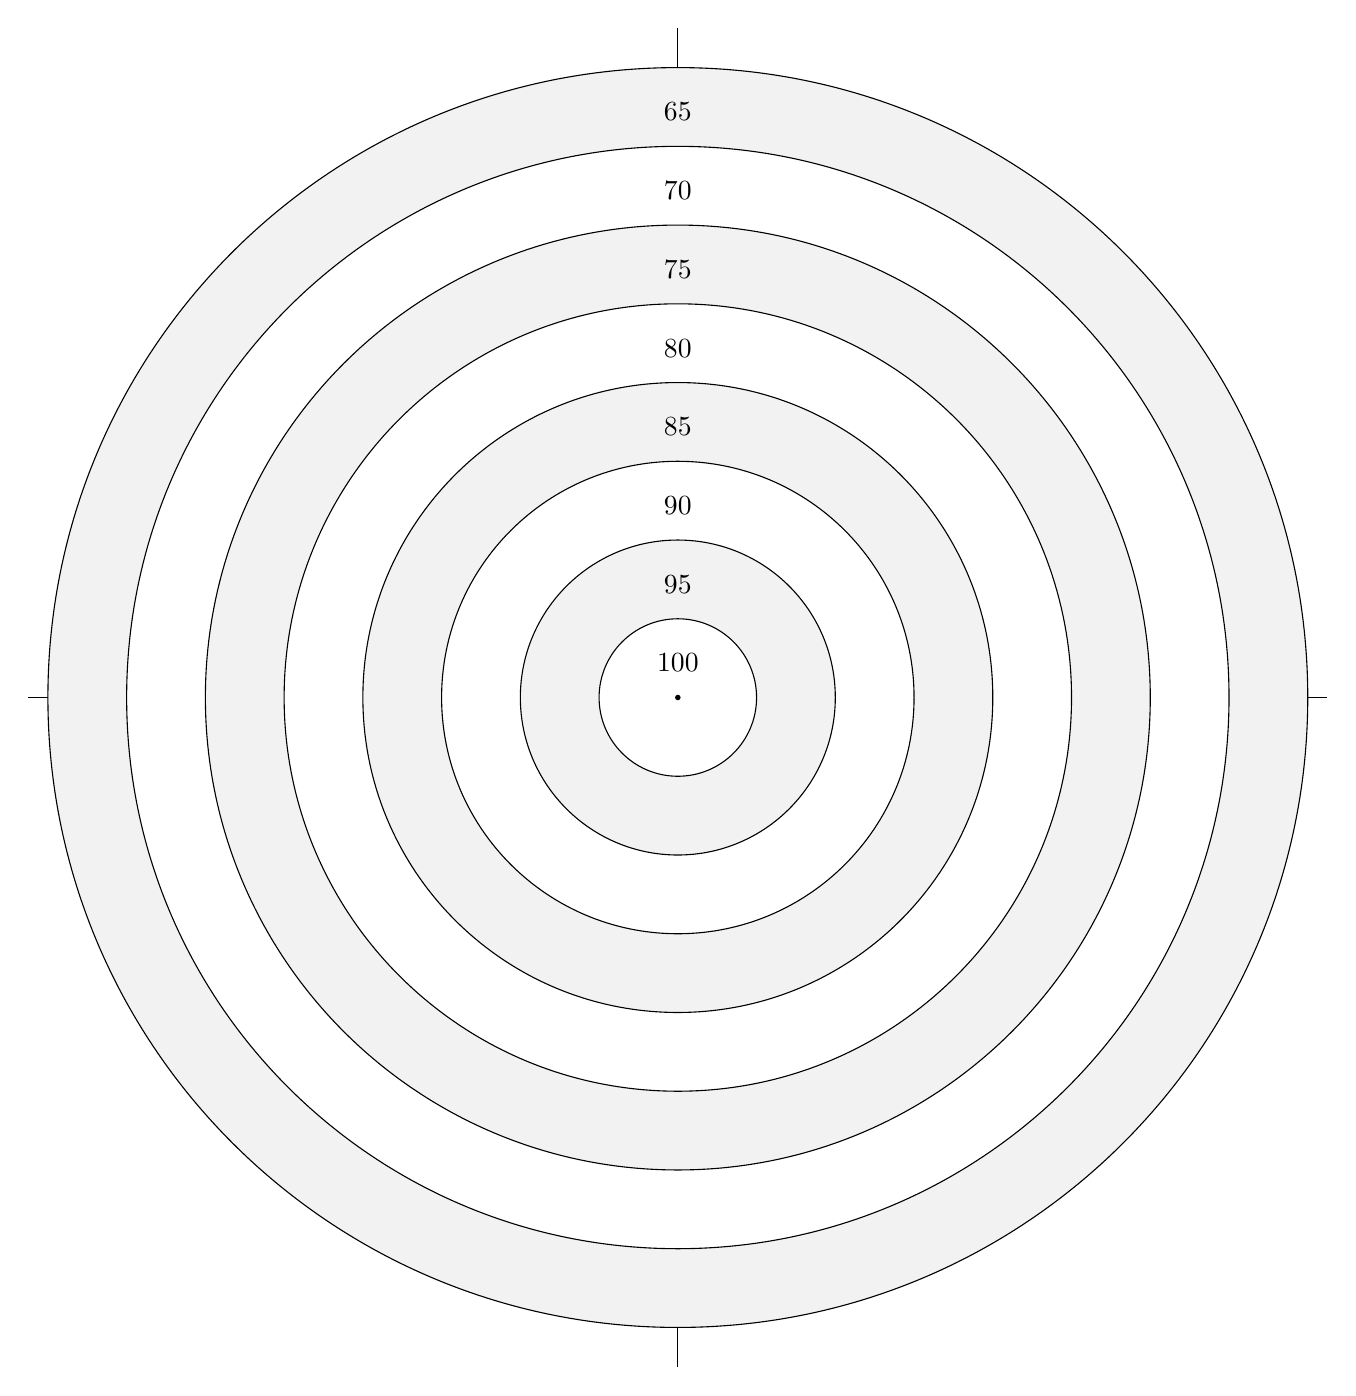
\begin{tikzpicture}
    \draw (-8.25,0) -- (8.25,0);
    \draw (0,8.5) -- (0,-8.5);   
    \draw[fill=black!5] (0,0) circle (8*1) node[above=7.2cm] {65};
    \draw[fill=white] (0,0) circle (7*1) node[above=6.2cm] {70};
    \draw[fill=black!5] (0,0) circle (6*1) node[above=5.2cm] {75};
    \draw[fill=white] (0,0) circle (5*1) node[above=4.2cm] {80};
    \draw[fill=black!5] (0,0) circle (4*1) node[above=3.2cm] {85};
    \draw[fill=white] (0,0) circle (3*1) node[above=2.2cm] {90};
    \draw[fill=black!5] (0,0) circle (2*1) node[above=1.2cm] {95};
    \draw[fill=white] (0,0) circle (1*1) node[above=0.2cm] {100};
    \fill (0,0) circle (1pt);
\end{tikzpicture}
\end{center}
\vspace*{\fill}

\clearpage

\subsection{Circular Motion}

\subsubsection{Uniform Circular Motion Using Multiple Representations}

\subsubsection{Quantities of Circular Motion}




\begin{questions}

% \question 
% Bring Figure to life by taking the following steps:


% \begin{enumerate}
%     \item Access the OpenStax Simulations (\href{https://veillette.github.io/simulations/}{click here}).
%     \item Click the simulation called ``Ladybug Motion.''
%     \item Under \texttt{Vectors}, check the boxes for \texttt{Show Velocity} and \texttt{Show Acceleration}. 
%     \item Towards the bottom, click \texttt{Velocity}. Then, under \texttt{Remote Control}, drag the red button until you generate a red arrow about 1 centimeter in length. The Ladybug will start moving.
%     \item When the Ladybug is in motion, locate the \texttt{Motion} options, and select \texttt{Circular}. The Ladybug is now undergoing uniform circular motion.
%     \item Draw a sketch of the Ladybug and its velocity and acceleration vectors. Compare your sketch to Figure \ref{4QmpMJ}. 
% \end{enumerate}

\question
If you attached a ball to a rope and swing it at a constant speed in a circle above your head, the ball is in uniform circular motion.

\begin{parts}
\part In which direction does it accelerate?
\part What force causes the acceleration?
\end{parts}

\question
In the diagram below, a car makes a sharp left turn. Draw a vector (an arrow) showing the direction of the centripetal force on the car making the left turn.

\begin{center}
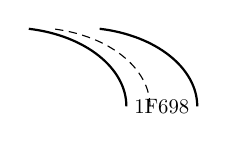
\begin{tikzpicture}
    \node at (1.65,0) {\resizebox{0.7cm}{!}{\usym{1F698}}};
    \draw[densely dashed,x=1.5cm] (1,0) arc (0:80:1);
    \draw[thick,x=1.5cm] (0.8,0) arc (0:80:1);
    \draw[thick,x=1.5cm] (1.4,0) arc (0:80:1);
\end{tikzpicture}
\end{center}

\question 
A runner moving at a speed of \SI{8.8}{m/s} rounds a bend with a radius of \SI{25}{m}. What is the centripetal acceleration of the runner?

\begin{solution}
\begin{equation*}
    a_c = \frac{v^2}{r} = \SI{3.1}{m/s^2}
\end{equation*}
\end{solution}

\question
Racing on a flat track, a car going \SI{32}{m/s} rounds a curve \SI{56}{m} in radius. What is the car's centripetal acceleration?

\begin{solution}
\begin{equation*}
    a_c = \frac{v^2}{r} = \SI{18.3}{m/s^2}
\end{equation*}
\end{solution}

\question
An airplane traveling at \SI{201}{m/s} makes a turn. What is the radius of the circular path if the pilot keeps the centripetal acceleration at \SI{5}{m/s^2}.

\begin{solution}
\begin{equation*}
    a_c = \frac{v^2}{r}
\end{equation*}

\begin{equation*}
    r = \frac{v^2}{a_c} = \SI{8080}{m}
\end{equation*}
\end{solution}

\question \label{x2YCzr} %1
What is meant by the word \textit{centripetal}?

\begin{solution}
Center-seeking
\end{solution}


\question \label{S4rGIt} %2
\begin{parts}
\part What is the direction of the velocity of an object in uniform circular motion?

\begin{solution}
tangent to the circular path
\end{solution}
\part What is the direction of the acceleration?

\begin{solution}
radially inward
\end{solution}
\end{parts}




\question \label{kTvEZX} %4
What is the centripetal acceleration felt by the passengers of a car moving at \SI{12}{m/s} along a curve with radius \SI{2.0}{m}?

\begin{solution}
\SI{72}{m/s^2}
\end{solution}




\question \label{fsjtBV} %6
Which of the following quantities is constant in uniform circular motion?

\begin{randomizechoices}
    \correctchoice speed
    \choice velocity
    \choice acceleration
    \choice displacement    
\end{randomizechoices}







\question \label{5lauZ6} %9
What happens to centripetal acceleration as the radius of curvature \textit{decreases} and the speed is held constant? Why?

\begin{solution}
Acceleration is inversely proportional to radius. Therefore, assuming speed stays the same, as radius \textit{decreases} (as the circle gets smaller), acceleration \textit{increases}. See Exercise \ref{aVu3ZA}.
\end{solution}


\question \label{KB7t4k} %10
Why do we experience more sideways acceleration while driving around sharper curves?

\begin{solution}
Sharper curve means smaller radius of curvature. As radius decreases, acceleration increases. See Exercise \ref{5lauZ6}.
\end{solution}


\question \label{jb3iGO} %11
Is centripetal acceleration a vector or a scalar?

\begin{solution}
vector
\end{solution}


\question \label{TUxTQh} %12
What are the units of centripetal acceleration?

\begin{solution}
meters per second squared (\SI{}{m/s^2})
\end{solution}





\question \label{IAjJBC} %17
An object in uniform circular motion moves at a constant speed. Is the object accelerating? Why or why not?

\begin{solution}
Yes. Although the object is not speeding up or slowing down, the direction of the velocity vector continuously changes. The acceleration vector points towards the center of the circular path and has magnitude $v^2/r$.
\end{solution}





%%%%%%%%%%%%%% FORCE %%%%%%%%%%%%%%%

\question \label{9YKhPo} %13
What are the units of centripetal force?

\begin{solution}
newton (N)
\end{solution}

\question \label{aVu3ZA} %3
Suppose you have an object tied to a rope and are rotating it over your head in uniform circular motion. If you increase the length of the rope, would you have to apply more force or less force to maintain the same speed?

\begin{solution}
Less force. In the centripetal force equation, the radius (the length of the rope) is in the denominator of the fraction. This means that force and radius are \textit{inversely proportional}: if one goes up, the other goes down. By \textit{increasing} the radius (the length of the rope), the centripetal force must \textit{decrease}.
\end{solution}

\question \label{MJm5VE} %5
Find the frictional force between the tires and the road that allows a \SI{1000}{kg} car traveling at \SI{30}{m/s} to round a \SI{20}{m} radius curve.

\begin{solution}
\SI{45000}{N}
\end{solution}

\question \label{GD8Yff} %7
List the three physical quantities that influence centripetal force.

\begin{solution}
Mass, speed, and radius.
\end{solution}

\question \label{aEtlVz} %8
An increase in the magnitude of the \fillin[radius of curvature][5cm] causes a \textit{decrease} in the centripetal force.

\begin{solution}
radius of curvature
\end{solution}

\question \label{wS6Htw} %14
What is the angle formed between the vectors of tangential velocity and centripetal force?

\begin{solution}
\SI{90}{\degree}
\end{solution}


\question \label{barV9C} %15
What is the angle formed between the vectors of centripetal acceleration and centripetal force?

\begin{solution}
\SI{0}{\degree}
\end{solution}


\question \label{M6NkHB} %16
As the mass of an object in uniform circular motion increases, what happens to the centripetal force required to keep it moving at the same speed?

\begin{solution}
Centripetal force must increase. Force and mass are \textit{directly proportional}: if one increases, the other goes increases too.
\end{solution}

\question \label{G8I4Up} %18
An object is in uniform circular motion. Suppose the centripetal force was removed. In which direction would the object now travel?

\begin{solution}
In the direction of the tangential velocity at the instant the force was removed.
\end{solution}


\question \label{Kv8Old} %19
An 89-kg system consisting of a bicycle and rider are rounding a turn at \SI{16}{m/s} on a path with a radius of curvature of \SI{25}{m}. 

\begin{parts}
\part What is the centripetal acceleration on the system?

\begin{solution}
\SI{10.24}{m/s^2}
\end{solution}

\part What is the centripetal force?

\begin{solution}
\SI{911}{N}
\end{solution}
\end{parts}




\end{questions}


\subsection{Circular Motion and Orbiting Bodies}

\subsubsection{How Radius and Mass Affects Orbiting Systems}

\subsection{Other}

\begin{questions}

\question
The $x$-component is the \fillin\ component of a vector.

\begin{choices}
    \correctchoice horizontal
    \choice vertical
    \choice direction
    \choice magnitude
\end{choices}

\question
The $y$-component is the \fillin\ component of a vector?

\begin{choices}
    \choice horizontal
    \choice direction
    \choice magnitude
    \correctchoice vertical
\end{choices}


\begin{EnvUplevel}
\textbf{Refer to the figure below and answer the following questions.}
\end{EnvUplevel}

\begin{figure}[h!]
    \centering
\def\Ax{2}
\def\Ay{6}
\begin{tikzpicture}
\pgfplotsset{compat=1.11}
    \begin{axis}[width=8cm,height=8cm,
        axis lines = middle,
        xlabel = $x$, x label style={anchor=west},
        ylabel = $y$, y label style={anchor=south},
        ymin=-8, ymax=8,
        xmin=-8, xmax=8,
        xtick={-8,-6,...,8},
        ytick={-8,-6,...,8},
        ymajorgrids=true,
        xmajorgrids=true,
        clip=false,
        ]
        \draw[ultra thick,red,->] (axis cs: 0,0) -- (\Ax,\Ay) node[red,above] {$\vec{A}$};
    \end{axis}
\end{tikzpicture}
\end{figure}

\question
What is the $x$-component of vector $\vec{A}$?

\begin{choices}
    \choice $-6$
    \choice $-2$
    \choice 6
    \correctchoice 2
\end{choices}

\question
What is the $y$-component of $\vec{A}$?

\begin{choices}
    \choice 2
    \correctchoice 6
    \choice $-2$
    \choice $-6$
\end{choices}
\vspace{1em}
\hrule



\clearpage
\begin{EnvUplevel}
\textbf{Read the passage below. Then answer the following questions.}

The fox travels 48 meters west, then makes a left and travels 55 meters south.
\end{EnvUplevel}

\question
 What is the magnitude of the fox's resultant displacement? (\textit{Tip}: Draw a sketch.)

\begin{choices}
    \choice \SI{48}{m}
    \choice \SI{55}{m}
    \choice \SI{103}{m}
    \correctchoice \SI{73}{m}
\end{choices}

\question
What is the direction of the resultant displacement as measured counter-clockwise from \SI{0}{\degree} (i.e., from the east axis)?

\begin{choices}
    \correctchoice \SI{229}{\degree}
    \choice \SI{194}{\degree}
    \choice \SI{48.9}{\degree}
    \choice \SI{304}{\degree}
\end{choices}
\vspace{1em}
\hrule

\begin{EnvUplevel}
    \textbf{Read the passage below. Then answer the remaining questions.}
    
    Sam Houston fires a cannon horizontally at \SI{63}{m/s} from the top of a tall cliff. The cliff is 754 meters tall.
\end{EnvUplevel}

\begin{figure}[h!]
    \centering
    \begin{tikzpicture} 
    \tikzmath{
        \gravity = 9.8;
        \vi = 28.6;
        \yi = 60;
        \thetai = 0.0;
        \ys = 1.3;
        \x1 = 20; \y1 = 57.60;
        \x2 = 40; \y2 = 50.42;
        \x3 = 60; \y3 = 38.43;
        \x4 = 80; \y4 = 21.66;
        \x5 = \vi*sqrt(2*\yi/\gravity); \y5 = 0;
    }
    \pgfplotsset{compat=1.11}
        \begin{axis}[width=8cm,height=8cm,ticks=none,
        axis line style = {black!50},
        axis lines = middle,
        clip=false,
        ylabel style= {anchor=south},
        xlabel style= {anchor=west},
        ylabel = $y$,
        xlabel = $x$,
        xmin=0, xmax=120,
        ymin=0, ymax=80,
        ]
        \addplot [dashed,
            domain=0:100,
            samples=100, 
            color=black!50,
        ]
        {\yi + tan(\thetai)*x - \gravity*x^2/(2*(\vi*cos(\thetai))^2)}; %equation of path
        \fill (0,\yi) circle (3pt) node[left] {$y_0$};
        \fill (\x1,\y1) circle (3pt); %Calculated using equator of path
        \fill (\x2,\y2) circle (3pt);
        \fill (\x3,\y3) circle (3pt);
        \fill (\x4,\y4) circle (3pt);
        \fill (\x5,\y5) circle (3pt);
        \end{axis}
    \end{tikzpicture}
\end{figure}

\question
What is the horizontal acceleration of the cannon?

\begin{choices}
    \correctchoice \SI{0}{m/s^2}
    \choice \SI{63}{m/s^2}
    \choice \SI{9.8}{m/s^2}
    \choice Unknown without time $t$
\end{choices}

\question
What is the cannon's vertical acceleration?

\begin{choices}
    \choice \SI{0}{m/s^2}
    \choice \SI{-63}{m/s^2}
    \correctchoice \SI{-9.8}{m/s^2}
    \choice Unknown without time $t$
\end{choices}

\clearpage
\question
What is the horizontal velocity of the cannon 4 seconds after launch?

\begin{choices}
    \correctchoice \SI{63}{m/s}
    \choice \SI{252}{m/s}
    \choice \SI{164}{m/s}
    \choice \SI{0}{m/s}
\end{choices}

\question 
What is the cannon's vertical velocity 4 seconds after launch?

\begin{choices}
    \choice \SI{-63.0}{m/s}
    \correctchoice \SI{-39.2}{m/s}
    \choice \SI{-105}{m/s}
    \choice \SI{-44.1}{m/s}
\end{choices}

\question
What is the cannon's horizontal displacement after 7 seconds of travel?

\begin{choices}
    \correctchoice \SI{441}{m}
    \choice \SI{63}{m}
    \choice \SI{867}{m}
    \choice \SI{225}{m}
\end{choices}

\question
What is the vertical displacement of the cannon 7 seconds after launch?

\begin{choices}
    \choice \SI{-34.4}{m}
    \choice \SI{-96}{m}
    \correctchoice \SI{-240}{m}
    \choice \SI{-390}{m}
\end{choices}


\question
How much time does it take the cannon to impact the ground below?

\begin{choices}
    \correctchoice \SI{12.4}{s}
    \choice \SI{13.0}{s}
    \choice \SI{14.1}{s}
    \choice \SI{15.2}{s}
\end{choices}

\question
What is the magnitude of the cannon's velocity as the cannon strikes the ground? (This is known as the ``entry speed.'')

\begin{choices}
    \choice \SI{58.6}{m/s}
    \correctchoice \SI{136.9}{m/s}
    \choice \SI{184.6}{m/s}
    \choice \SI{7658}{m/s}
\end{choices}




\clearpage
\question
After takeoff, an airplane travels \SI{120}{m} at \SI{33}{\degree} above the horizontal. What is the horizontal component of its displacement?

\begin{choices}
    \choice \SI{65.4}{m}
    \choice \SI{98.0}{m}
    \correctchoice \SI{101}{m}
    \choice \SI{3960}{m}
\end{choices}

\question
For the airplane in the previous problem, what is the vertical displacement?

\begin{choices}
    \choice \SI{101}{m}
    \choice \SI{75.4}{m}
    \choice \SI{33.0}{m}
    \correctchoice \SI{65.4}{m}
\end{choices}


\begin{EnvUplevel}
\textbf{Refer to the figure below and answer the following questions.}
\end{EnvUplevel}

\begin{figure}[h!]
    \centering
\def\A{5}
\def\angle{142}
\begin{tikzpicture}
\pgfplotsset{compat=1.11}
\begin{axis}[width=8cm,height=8cm,
    axis lines=middle,
    axis line style={black!20},
    xmin=-5,xmax=5,ymin=-5,ymax=5,
    axis equal,
    ticks = none,
    xlabel = $x$, x label style={anchor=west},
    ylabel = $y$, y label style={anchor=south},
        ticks=none,
        clip=false,
        ]
        \node[left] at (axis cs: -5,0) {$-x$};
        \node[below] at (axis cs: 0,-5) {$-y$};
        \draw[thick] (axis cs: -1,0) arc (180:\angle:1);
        \node at (axis cs: -1.8,0.5) {\SI{38}{\degree}}; %180 - 142 = 38
        \draw[ultra thick,black,->] (axis cs: 0,0) -- ++(axis direction cs: {\A*cos(\angle)},{\A*sin(\angle)}) node[above] {$\vec{A}=16$};
    \end{axis}
\end{tikzpicture}
\end{figure}

\question
What is the $x$-component of the vector?

\begin{choices}
    \choice $-9.85$
    \choice 12.6
    \choice 9.85
    \correctchoice $-12.6$
\end{choices}

\question
What is the $y$-component of the vector?

\begin{choices}
    \choice 12.6
    \correctchoice 9.85
    \choice $-12.6$
    \choice $-9.85$
\end{choices}

\question
Memo, the goalkeeper, wants to kick a soccer ball as far down the field as possible. Which of the following launch angles will produce the largest horizontal displacement?

\begin{minipage}{6cm}
\centering
    \begin{randomizechoices}
        \correctchoice \ang{47}
        \choice \ang{86}
        \choice \ang{15}
        \choice \ang{39}
    \end{randomizechoices}
\end{minipage}%
\begin{minipage}{6cm}
    \begin{center}
        \begin{tikzpicture} 
        \tikzmath{
            \vi = 18.0;
            \yi = 0;
            \thetai = 70.0;
        }
        \tikzset{declare function={f(\x)=\yi + tan(\thetai)*\x - 9.8*\x^2/(2*(\vi*cos(\thetai))^2);}} %equation of path
        \pgfplotsset{compat=1.11}
            \begin{axis}[width=7cm,height=6cm,ticks=none,
            axis lines = center,
            clip=false,
            ylabel = $y$,
            xlabel = $x$,
            xmin=0, xmax=20,
            ymin=0, ymax=18,
            % axis line style={draw=none},
            ]
            \draw[dashed,domain=0:16,variable=\x,samples=200] plot ({\x},{f(\x)}) node {\faSoccerBallO};
            \draw (1.5,0) arc (0:60:1.5) node[right=2pt,pos=0.8] {$\theta$};
            \end{axis}
        \end{tikzpicture}
        \label{i1Y7vV}
    \end{center}
\end{minipage}

\question
What is the angle between the $x$ and $y$ components of a vector?

\begin{randomizechoices}
    \correctchoice \ang{90}
    \choice \ang{45}
    \choice \ang{0}
    \choice \ang{30}
\end{randomizechoices}

\question
True or False? Range is defined as the maximum vertical distance travelled by a projectile. 

\begin{choices}
    \choice True
    \correctchoice False
\end{choices}

\question
For what angle of a projectile is its range equal to zero?

\begin{randomizechoices}
    \correctchoice \ang{90}
    \choice \ang{45}
    \choice \ang{10}
    \choice \ang{1}
\end{randomizechoices}

\clearpage
\question
On November 5, 2022, Yordan Alvarez of the Houston Astros hit a game-winning home run at Minute Maid Park. The baseball was hit with an exit velocity of \SI{50.3}{m/s} at a launch angle of \ang{27}. When the ball's horizontal displacement from the plate was 110 meters, its height above ground was 26.5 meters. Calculate the ball's displacement from home plate at this instant.

\vspace{1em}

\begin{minipage}{6cm}
    \centering 
    \begin{randomizechoices}
        \correctchoice \SI{113}{m}
        \choice \SI{110}{m}
        \choice \SI{136}{m}
        \choice \SI{12803}{m}
    \end{randomizechoices}
\end{minipage}%
\begin{minipage}{6cm}
    \centering 
    \begin{center}
        \begin{tikzpicture} 
        \tikzmath{
            \vi = 50.3;
            \yi = 0;
            \thetai = 27.0;
        }
        \tikzset{declare function={f(\x)=\yi + tan(\thetai)*\x - 9.8*\x^2/(2*(\vi*cos(\thetai))^2);}} %equation of path
        \pgfplotsset{compat=1.11}
        \begin{axis}[width=6cm,height=6cm,ticks=none,
            axis lines = center,
            clip=false,
            axis equal image,
            xmin=0, xmax=120,
            ymin=0, ymax=40,
            axis line style={draw=none},
            ticks=none,
            ]
            \draw[lightgray,domain=0:110,variable=\x,samples=200] plot ({\x},{f(\x)});
            \draw[->,thick] (0,0) -- ++(110,{f(110)}) node[pos=0.75,below]{$d$};
            \draw[->,dashed] (0,0) -- ++(110,0) node[pos=0.5,below] {\SI{110}{m}};
            \draw[->,dashed] (110,0) -- ++(0,{f(110)}) node[pos=0.5,right] {\SI{26.5}{m}};
            \draw[fill=black] (110,{f(110)}) circle (2pt);
            \end{axis}
        \end{tikzpicture}
    \end{center}    
\end{minipage}%

\question
The Harbinger Willow Tail is a comet-like firework shell that makes for an awesome spectacle. It's launched with horizontal and vertical velocity components of \SI{20.6}{m/s} and \SI{51.0}{m/s}, respectively. How much time after launch will it take the Harbinger to reach its maximum height?

\begin{randomizechoices}
    \correctchoice \SI{5.2}{s}
    \choice \SI{6.9}{s}
    \choice \SI{4.8}{s}
    \choice \SI{7.3}{s}
\end{randomizechoices}



\clearpage

\question \label{EJzjXh}
The JPMorgan Chase Tower is the tallest building in Houston, at a height of 305 meters. If Tiger Woods horizontally launches a golf ball at 12 meters per second off the roof, how long will it take the ball to strike the ground? Ignore air resistance.

\begin{minipage}{6cm}
    \centering
    \begin{randomizechoices}
        \correctchoice \SI{7.9}{s}
        \choice \SI{5.6}{s}
        \choice \SI{1.6}{s}
        \choice \SI{3.9}{s}
    \end{randomizechoices}
\end{minipage}%
\begin{minipage}{6cm}
    \centering
    \begin{center}
        \begin{tikzpicture}[
                declare function={f(\x,\yi,\vi,\thetai)=\yi + tan(\thetai)*\x - \grav*\x^2/(2*(\vi*cos(\thetai))^2);}, %equation of path
                declare function ={R(\vi,\thetai)= \vi^2*sin(2*\thetai)/\grav;}, %range
                declare function={h(\vi,\thetai)=(\vi*sin(\thetai))^2/(2*\grav);}, %maximum height
            ]
            \tikzmath{
                \grav = 9.8;
                \sf = 0.5; %scale factor for vector components
            }
        \pgfplotsset{compat=1.11}
            \begin{axis}[width=6cm,height=6cm,ticks=none,
            axis lines = center,
            clip=false,
            xmin=0, xmax=150,
            ymin=0, ymax=350,
            axis line style={draw=none}
            ]
            \draw[dashed,domain=0:95,variable=\x,samples=100] plot ({\x},{f(\x,305,12,0)});
            \begin{scope}[shift={(-20,0)}]
                \draw[fill=black!50] (0,0) rectangle (20,305);
            \end{scope}
            \end{axis}
        \end{tikzpicture}
    \end{center}
\end{minipage}

\question
How does the elapsed time from Question \ref{EJzjXh} change if the ball is dropped vertically from rest instead of launched horizontally?

\begin{randomizechoices}[keeplast]
    \correctchoice The new elapsed time remains the same.
    \choice The new elapsed time is longer.
    \choice The new elapsed time is shorter.
    \choice It's impossible to determine.
\end{randomizechoices}



\end{questions}

\end{document}


